% Very simple template for lab reports. Most common packages are already included.
\documentclass[a4paper, 11pt]{article}
\usepackage[utf8]{inputenc} % Change according your file encoding
\usepackage{graphicx}
\usepackage{url}
\usepackage{listings}
\usepackage[listings]{tcolorbox}
\usepackage{xcolor}
\usepackage{xcolor}
\usepackage{float} 
\usepackage{placeins} 

% Define a custom boxed listing environment
\newtcblisting{mylisting}{
  colback=gray!5!white, colframe=black!75!white,
  listing only,
  left=2mm, right=2mm, top=1mm, bottom=1mm,
  boxrule=0.5pt, arc=2mm
}

%opening
\title{Report 3 - Routy: A Logical Time Logger}
\author{Lorenzo Deflorian}
\date{\today{}}

\begin{document}

\maketitle

\section{Introduction}

The main goal of this assignment was to implement a logger that uses logical time to order messages in a distributes system. The logger should be able to handle messages that are received out of order and log them in the correct order based on their logical timestamps.

For this purpose I have implemented both a lamport clock and a vector clock. The lamport clock is a simple counter starting from 0 that is incremented every time a message is sent or received. The vector clock is a map that keeps track of the logical time of each node in the system. Every time a message is sent, the sender increments its own clock and includes the updated clock in the message. When a message is received, the receiver updates its own clock by taking the maximum of its own clock and the received clock.

To log the messages in the correct order, I have also implemented a holdback queue that store the messages the are considered unsafe to be logged. A message is considered safe to be logged if its timestamp is less than or equal to all the timestamps that the logger keeps track of. At every iteration the logger checks the holdback queue for any messages that can be logged and logs them in the correct order.


\section{Main problems and solutions}

\subsection{Logging wrong in the order}

After implementing the basic functionality of the logger running the test with a high Jitter (300ms) immediatly showed that without a holdback queue the logger was not able to log the messages in the correct order. This can be easly seen looking for entries like the following in the log file:
\begin{tcolorbox}[colback=black!5!white, colframe=black!80!white, title=Log Output, fonttitle=\bfseries, sharp corners=south, listing only]
\begin{verbatim}
log: 2 george {received,{hello,83}}
log: 1 paul {sending,{hello,83}}
log: 4 john {received,{hello,15}}
log: 2 paul {sending,{hello,93}}
log: 5 john {received,{hello,53}}
log: 3 george {sending,{hello,15}}
log: 4 george {received,{hello,93}}
log: 1 ringo {sending,{hello,53}}
log: 6 john {received,{hello,30}}
log: 8 george {received,{hello,81}}
log: 10 ringo {received,{hello,12}}
log: 3 paul {sending,{hello,30}}
log: 7 john {sending,{hello,81}}
log: 9 george {sending,{hello,12}}
log: 11 ringo {received,{hello,35}}
log: 11 john {received,{hello,29}} <--- OUT OF ORDER
log: 4 paul {sending,{hello,35}}
log: 13 john {received,{hello,74}}
log: 10 george {sending,{hello,29}} <--- OUT OF ORDER
log: 15 paul {received,{hello,24}}
log: 11 george {sending,{hello,69}}
log: 12 ringo {sending,{hello,74}}
log: 14 john {sending,{hello,24}}
log: 15 john {received,{hello,69}}
log: 16 john {received,{hello,25}}
\end{verbatim}
\end{tcolorbox}

As we can see pairing the sending and receiving message, the order is not respected for 
message \{hello,29\} that is first being received and then sent. 

\begin{table}[H]
\centering
\begin{tabular}{|l|l|c|l|c|c|}
\hline
\textbf{Message} & \textbf{Sender} & \textbf{Send Time} & \textbf{Receiver} & \textbf{Receive Time} & \textbf{Ordered?} \\
\hline
\{hello,83\}  & paul   & 1  & george & 2  & Yes \\
\{hello,15\}  & george & 3  & john   & 4  & Yes \\
\{hello,93\}  & paul   & 2  & george & 4  & Yes \\
\{hello,53\}  & ringo  & 1  & john   & 5  & Yes \\
\{hello,30\}  & paul   & 3  & john   & 6  & Yes \\
\{hello,81\}  & john   & 7  & george & 8  & Yes \\
\{hello,12\}  & george & 9  & ringo  & 10 & Yes \\
\{hello,35\}  & paul   & 4  & ringo  & 11 & Yes \\
\{hello,74\}  & ringo  & 12 & john   & 13 & Yes \\
\{hello,29\}  & george & 10 & john   & 11 & No  \\
\{hello,69\}  & george & 11 & john   & 15 & Yes \\
\{hello,24\}  & john   & 14 & paul   & 15 & Yes \\
\hline
\end{tabular}
\caption{Message send and receive times with validity}
\end{table}

Even tho the send and receive are logged in the wrong order, the timestamps respect casuality! This means that nevertheless the logical clock is working correctly.

\subsection{Hold my Logs}

Let's implement a holdback queue to store unsafe messages and only log the same ones.
At the beginning of every iteration the logger check the holdback queue for any messages that can be logged and logs them in the correct order. When the logger receives a message it checks if the message is safe to be logged, if it is it logs it, otherwise it adds it to the holdback queue. When in the end the logger receives a stop message it logs all the remaining messages in the holdback queue.

Let's see how many messages are stored in the holdback queue during the execution of the test with a high jitter (300ms) between 50 nodes. Note that for the following test I have modified the message ID to be a random number between 1 and 1,000,000 instead of between 1 and 100. This is to reduce the probability of having two messages with the same ID.

\begin{figure}[H]
  \centering
  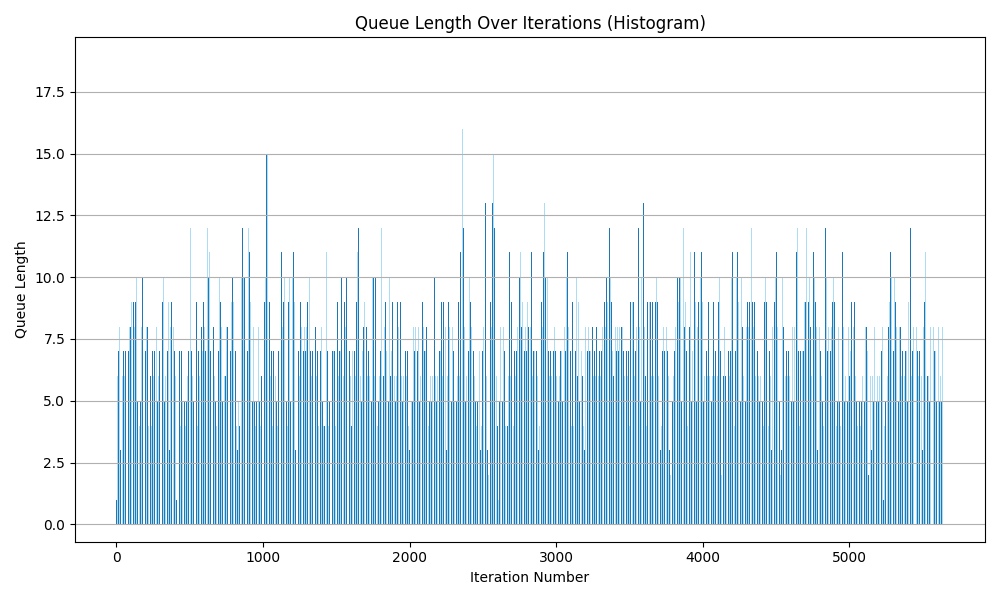
\includegraphics[width=0.8\textwidth]{imgs/test_queue_len_50_histogram.png}
  \caption{Histogram of holdback queue length during execution with 50 nodes and 300ms jitter}
  \label{fig:queue_histogram}
\end{figure}

As we can see from the histogram in figure \ref{fig:queue_histogram}, the holdback queue length is mostly between 0 and 5 messages, with a few peaks reaching up to 17 messages. This means that the logger is able to log most of the messages in the correct order without having to store them in the holdback queue for too long.

\subsection{V for Vector}
To further improve the logging order I have implemented a vector clock. The vector clock is a map that keeps track of the logical time of each node in the system. Every time a message is sent, the sender increments its own clock and includes the updated clock in the message. When a message is received, the receiver updates its own clock by taking the maximum of its own clock and the received clock.

Using the script \texttt{check\_vector.py}, I have verified that the vector clock is working correctly and that the messages are logged in the correct order.

Sometimes it happens that a message appears to received without being sent first. This happens because of the Jitter introduced between the Send and the Log call. Anyhow this doesn't affect the correctness of the logging order or the causality of the messages.

\section{Conclusions}

To wrap it up I have implemented a logger that uses logical time to order messages in a distributed system. The logger is able to handle messages that are received out of order and log them in the correct order based on their logical timestamps. The implementation of a holdback queue and a vector clock further improves the logging order and ensures that the messages are logged in a causally consistent manner.

For further improvements we could handle a better way of generating unique message IDs to avoid collisions. We could also implement a more efficient way of checking the holdback queue for safe messages to log, for example by using a priority queue.

\end{document}